\documentclass[1p]{elsarticle_modified}
%\bibliographystyle{elsarticle-num}

%\usepackage[colorlinks]{hyperref}
%\usepackage{abbrmath_seonhwa} %\Abb, \Ascr, \Acal ,\Abf, \Afrak
\usepackage{amsfonts}
\usepackage{amssymb}
\usepackage{amsmath}
\usepackage{amsthm}
\usepackage{scalefnt}
\usepackage{amsbsy}
\usepackage{kotex}
\usepackage{caption}
\usepackage{subfig}
\usepackage{color}
\usepackage{graphicx}
\usepackage{xcolor} %% white, black, red, green, blue, cyan, magenta, yellow
\usepackage{float}
\usepackage{setspace}
\usepackage{hyperref}

\usepackage{tikz}
\usetikzlibrary{arrows}

\usepackage{multirow}
\usepackage{array} % fixed length table
\usepackage{hhline}

%%%%%%%%%%%%%%%%%%%%%
\makeatletter
\renewcommand*\env@matrix[1][\arraystretch]{%
	\edef\arraystretch{#1}%
	\hskip -\arraycolsep
	\let\@ifnextchar\new@ifnextchar
	\array{*\c@MaxMatrixCols c}}
\makeatother %https://tex.stackexchange.com/questions/14071/how-can-i-increase-the-line-spacing-in-a-matrix
%%%%%%%%%%%%%%%

\usepackage[normalem]{ulem}

\newcommand{\msout}[1]{\ifmmode\text{\sout{\ensuremath{#1}}}\else\sout{#1}\fi}
%SOURCE: \msout is \stkout macro in https://tex.stackexchange.com/questions/20609/strikeout-in-math-mode

\newcommand{\cancel}[1]{
	\ifmmode
	{\color{red}\msout{#1}}
	\else
	{\color{red}\sout{#1}}
	\fi
}

\newcommand{\add}[1]{
	{\color{blue}\uwave{#1}}
}

\newcommand{\replace}[2]{
	\ifmmode
	{\color{red}\msout{#1}}{\color{blue}\uwave{#2}}
	\else
	{\color{red}\sout{#1}}{\color{blue}\uwave{#2}}
	\fi
}

\newcommand{\Sol}{\mathcal{S}} %segment
\newcommand{\D}{D} %diagram
\newcommand{\A}{\mathcal{A}} %arc


%%%%%%%%%%%%%%%%%%%%%%%%%%%%%5 test

\def\sl{\operatorname{\textup{SL}}(2,\Cbb)}
\def\psl{\operatorname{\textup{PSL}}(2,\Cbb)}
\def\quan{\mkern 1mu \triangleright \mkern 1mu}

\theoremstyle{definition}
\newtheorem{thm}{Theorem}[section]
\newtheorem{prop}[thm]{Proposition}
\newtheorem{lem}[thm]{Lemma}
\newtheorem{ques}[thm]{Question}
\newtheorem{cor}[thm]{Corollary}
\newtheorem{defn}[thm]{Definition}
\newtheorem{exam}[thm]{Example}
\newtheorem{rmk}[thm]{Remark}
\newtheorem{alg}[thm]{Algorithm}

\newcommand{\I}{\sqrt{-1}}
\begin{document}

%\begin{frontmatter}
%
%\title{Boundary parabolic representations of knots up to 8 crossings}
%
%%% Group authors per affiliation:
%\author{Yunhi Cho} 
%\address{Department of Mathematics, University of Seoul, Seoul, Korea}
%\ead{yhcho@uos.ac.kr}
%
%
%\author{Seonhwa Kim} %\fnref{s_kim}}
%\address{Center for Geometry and Physics, Institute for Basic Science, Pohang, 37673, Korea}
%\ead{ryeona17@ibs.re.kr}
%
%\author{Hyuk Kim}
%\address{Department of Mathematical Sciences, Seoul National University, Seoul 08826, Korea}
%\ead{hyukkim@snu.ac.kr}
%
%\author{Seokbeom Yoon}
%\address{Department of Mathematical Sciences, Seoul National University, Seoul, 08826,  Korea}
%\ead{sbyoon15@snu.ac.kr}
%
%\begin{abstract}
%We find all boundary parabolic representation of knots up to 8 crossings.
%
%\end{abstract}
%\begin{keyword}
%    \MSC[2010] 57M25 
%\end{keyword}
%
%\end{frontmatter}

%\linenumbers
%\tableofcontents
%
\newcommand\colored[1]{\textcolor{white}{\rule[-0.35ex]{0.8em}{1.4ex}}\kern-0.8em\color{red} #1}%
%\newcommand\colored[1]{\textcolor{white}{ #1}\kern-2.17ex	\textcolor{white}{ #1}\kern-1.81ex	\textcolor{white}{ #1}\kern-2.15ex\color{red}#1	}

{\Large $\underline{12a_{0229}~(K12a_{0229})}$}

\setlength{\tabcolsep}{10pt}
\renewcommand{\arraystretch}{1.6}
\vspace{1cm}\begin{tabular}{m{100pt}>{\centering\arraybackslash}m{274pt}}
\multirow{5}{120pt}{
	\centering
	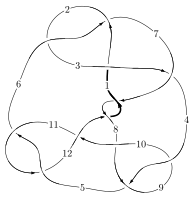
\includegraphics[width=112pt]{../../../GIT/diagram.site/Diagrams/png/1030_12a_0229.png}\\
\ \ \ A knot diagram\footnotemark}&
\allowdisplaybreaks
\textbf{Linearized knot diagam} \\
\cline{2-2}
 &
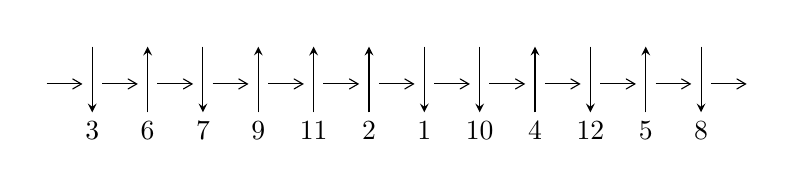
\begin{tikzpicture}[x=20pt, y=17pt]
	% nodes
	\node (C0) at (0, 0) {};
	\node (C1) at (1, 0) {};
	\node (C1U) at (1, +1) {};
	\node (C1D) at (1, -1) {3};

	\node (C2) at (2, 0) {};
	\node (C2U) at (2, +1) {};
	\node (C2D) at (2, -1) {6};

	\node (C3) at (3, 0) {};
	\node (C3U) at (3, +1) {};
	\node (C3D) at (3, -1) {7};

	\node (C4) at (4, 0) {};
	\node (C4U) at (4, +1) {};
	\node (C4D) at (4, -1) {9};

	\node (C5) at (5, 0) {};
	\node (C5U) at (5, +1) {};
	\node (C5D) at (5, -1) {11};

	\node (C6) at (6, 0) {};
	\node (C6U) at (6, +1) {};
	\node (C6D) at (6, -1) {2};

	\node (C7) at (7, 0) {};
	\node (C7U) at (7, +1) {};
	\node (C7D) at (7, -1) {1};

	\node (C8) at (8, 0) {};
	\node (C8U) at (8, +1) {};
	\node (C8D) at (8, -1) {10};

	\node (C9) at (9, 0) {};
	\node (C9U) at (9, +1) {};
	\node (C9D) at (9, -1) {4};

	\node (C10) at (10, 0) {};
	\node (C10U) at (10, +1) {};
	\node (C10D) at (10, -1) {12};

	\node (C11) at (11, 0) {};
	\node (C11U) at (11, +1) {};
	\node (C11D) at (11, -1) {5};

	\node (C12) at (12, 0) {};
	\node (C12U) at (12, +1) {};
	\node (C12D) at (12, -1) {8};
	\node (C13) at (13, 0) {};

	% arrows
	\draw[->,>={angle 60}]
	(C0) edge (C1) (C1) edge (C2) (C2) edge (C3) (C3) edge (C4) (C4) edge (C5) (C5) edge (C6) (C6) edge (C7) (C7) edge (C8) (C8) edge (C9) (C9) edge (C10) (C10) edge (C11) (C11) edge (C12) (C12) edge (C13) ;	\draw[->,>=stealth]
	(C1U) edge (C1D) (C2D) edge (C2U) (C3U) edge (C3D) (C4D) edge (C4U) (C5D) edge (C5U) (C6D) edge (C6U) (C7U) edge (C7D) (C8U) edge (C8D) (C9D) edge (C9U) (C10U) edge (C10D) (C11D) edge (C11U) (C12U) edge (C12D) ;
	\end{tikzpicture} \\
\hhline{~~} \\& 
\textbf{Solving Sequence} \\ \cline{2-2} 
 &
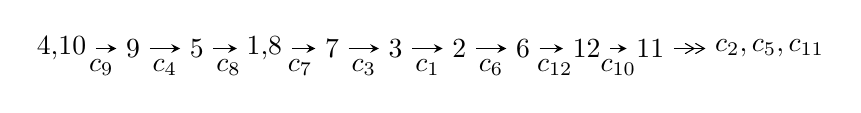
\begin{tikzpicture}[x=23pt, y=7pt]
	% node
	\node (A0) at (-1/8, 0) {4,10};
	\node (A1) at (1, 0) {9};
	\node (A2) at (2, 0) {5};
	\node (A3) at (49/16, 0) {1,8};
	\node (A4) at (33/8, 0) {7};
	\node (A5) at (41/8, 0) {3};
	\node (A6) at (49/8, 0) {2};
	\node (A7) at (57/8, 0) {6};
	\node (A8) at (65/8, 0) {12};
	\node (A9) at (73/8, 0) {11};
	\node (C1) at (1/2, -1) {$c_{9}$};
	\node (C2) at (3/2, -1) {$c_{4}$};
	\node (C3) at (5/2, -1) {$c_{8}$};
	\node (C4) at (29/8, -1) {$c_{7}$};
	\node (C5) at (37/8, -1) {$c_{3}$};
	\node (C6) at (45/8, -1) {$c_{1}$};
	\node (C7) at (53/8, -1) {$c_{6}$};
	\node (C8) at (61/8, -1) {$c_{12}$};
	\node (C9) at (69/8, -1) {$c_{10}$};
	\node (A10) at (11, 0) {$c_{2},c_{5},c_{11}$};

	% edge
	\draw[->,>=stealth]	
	(A0) edge (A1) (A1) edge (A2) (A2) edge (A3) (A3) edge (A4) (A4) edge (A5) (A5) edge (A6) (A6) edge (A7) (A7) edge (A8) (A8) edge (A9) ;
	\draw[->>,>={angle 60}]	
	(A9) edge (A10);
\end{tikzpicture} \\ 

\end{tabular} \\

\footnotetext{
The image of knot diagram is generated by the software ``\textbf{Draw programme}" developed by Andrew Bartholomew(\url{http://www.layer8.co.uk/maths/draw/index.htm\#Running-draw}), where we modified some parts for our purpose(\url{https://github.com/CATsTAILs/LinksPainter}).
}\phantom \\ \newline 
\centering \textbf{Ideals for irreducible components\footnotemark of $X_{\text{par}}$} 
 
\begin{align*}
I^u_{1}&=\langle 
- u^{45}- u^{44}+\cdots+64 b-1,\;- u^{45}- u^{44}+\cdots+64 a-65,\;u^{46}+9 u^{44}+\cdots+7 u^2+1\rangle \\
I^u_{2}&=\langle 
5.89603\times10^{55} u^{65}+1.20824\times10^{54} u^{64}+\cdots+8.65172\times10^{55} b-2.59504\times10^{56},\\
\phantom{I^u_{2}}&\phantom{= \langle  }-3.37617\times10^{56} u^{65}+7.20416\times10^{53} u^{64}+\cdots+1.47079\times10^{57} a+7.90685\times10^{57},\\
\phantom{I^u_{2}}&\phantom{= \langle  }u^{66}+u^{65}+\cdots-10 u+17\rangle \\
I^u_{3}&=\langle 
b- a-1,\;a^6+a^5 u+a^4+2 a^3 u+a u-1,\;u^2+1\rangle \\
\\
\end{align*}
\raggedright * 3 irreducible components of $\dim_{\mathbb{C}}=0$, with total 124 representations.\\
\footnotetext{All coefficients of polynomials are rational numbers. But the coefficients are sometimes approximated in decimal forms when there is not enough margin.}
\newpage
\renewcommand{\arraystretch}{1}
\centering \section*{I. $I^u_{1}= \langle - u^{45}- u^{44}+\cdots+64 b-1,\;- u^{45}- u^{44}+\cdots+64 a-65,\;u^{46}+9 u^{44}+\cdots+7 u^2+1 \rangle$}
\flushleft \textbf{(i) Arc colorings}\\
\begin{tabular}{m{7pt} m{180pt} m{7pt} m{180pt} }
\flushright $a_{4}=$&$\begin{pmatrix}0\\u\end{pmatrix}$ \\
\flushright $a_{10}=$&$\begin{pmatrix}1\\0\end{pmatrix}$ \\
\flushright $a_{9}=$&$\begin{pmatrix}1\\u^2\end{pmatrix}$ \\
\flushright $a_{5}=$&$\begin{pmatrix}u\\u^3+u\end{pmatrix}$ \\
\flushright $a_{1}=$&$\begin{pmatrix}0.0156250 u^{45}+0.0156250 u^{44}+\cdots+0.0156250 u+1.01563\\0.0156250 u^{45}+0.0156250 u^{44}+\cdots+0.0156250 u+0.0156250\end{pmatrix}$ \\
\flushright $a_{8}=$&$\begin{pmatrix}u^2+1\\u^2\end{pmatrix}$ \\
\flushright $a_{7}=$&$\begin{pmatrix}-\frac{9}{32} u^{45}-\frac{7}{32} u^{44}+\cdots-\frac{5}{16} u+\frac{3}{4}\\-0.265625 u^{45}-0.203125 u^{44}+\cdots-0.296875 u-0.234375\end{pmatrix}$ \\
\flushright $a_{3}=$&$\begin{pmatrix}0.546875 u^{45}-2.51563 u^{44}+\cdots+3.04688 u-4.82813\\\frac{3}{16} u^{45}-\frac{29}{16} u^{44}+\cdots+\frac{19}{8} u-\frac{15}{4}\end{pmatrix}$ \\
\flushright $a_{2}=$&$\begin{pmatrix}3.37500 u^{45}+2.65625 u^{44}+\cdots+3.84375 u+8.18750\\0.609375 u^{45}+2.07813 u^{44}+\cdots-1.32813 u+5.20313\end{pmatrix}$ \\
\flushright $a_{6}=$&$\begin{pmatrix}0.0156250 u^{45}-0.0156250 u^{44}+\cdots+2.01563 u-0.0156250\\u^5+u^3+u\end{pmatrix}$ \\
\flushright $a_{12}=$&$\begin{pmatrix}0.0156250 u^{45}+0.0156250 u^{44}+\cdots+0.0156250 u+1.01563\\- u^2\end{pmatrix}$ \\
\flushright $a_{11}=$&$\begin{pmatrix}0.0156250 u^{45}+0.0156250 u^{44}+\cdots+0.0156250 u+1.01563\\u^4\end{pmatrix}$\\&\end{tabular}
\flushleft \textbf{(ii) Obstruction class $= -1$}\\~\\
\flushleft \textbf{(iii) Cusp Shapes $= -\frac{105}{8} u^{45}-\frac{21}{16} u^{44}+\cdots-\frac{565}{16} u-\frac{113}{8}$}\\~\\
\newpage\renewcommand{\arraystretch}{1}
\flushleft \textbf{(iv) u-Polynomials at the component}\newline \\
\begin{tabular}{m{50pt}|m{274pt}}
Crossings & \hspace{64pt}u-Polynomials at each crossing \\
\hline $$\begin{aligned}c_{1}\end{aligned}$$&$\begin{aligned}
&u^{46}+21 u^{45}+\cdots+11 u+4
\end{aligned}$\\
\hline $$\begin{aligned}c_{2},c_{6}\end{aligned}$$&$\begin{aligned}
&u^{46}-3 u^{45}+\cdots-9 u+2
\end{aligned}$\\
\hline $$\begin{aligned}c_{3}\end{aligned}$$&$\begin{aligned}
&u^{46}+3 u^{45}+\cdots+107 u+10
\end{aligned}$\\
\hline $$\begin{aligned}c_{4},c_{5},c_{9}\\c_{11}\end{aligned}$$&$\begin{aligned}
&u^{46}+9 u^{44}+\cdots+7 u^2+1
\end{aligned}$\\
\hline $$\begin{aligned}c_{7},c_{12}\end{aligned}$$&$\begin{aligned}
&u^{46}-15 u^{45}+\cdots-1507 u+86
\end{aligned}$\\
\hline $$\begin{aligned}c_{8},c_{10}\end{aligned}$$&$\begin{aligned}
&u^{46}+18 u^{45}+\cdots+14 u+1
\end{aligned}$\\
\hline
\end{tabular}\\~\\
\newpage\renewcommand{\arraystretch}{1}
\flushleft \textbf{(v) Riley Polynomials at the component}\newline \\
\begin{tabular}{m{50pt}|m{274pt}}
Crossings & \hspace{64pt}Riley Polynomials at each crossing \\
\hline $$\begin{aligned}c_{1}\end{aligned}$$&$\begin{aligned}
&y^{46}+9 y^{45}+\cdots+223 y+16
\end{aligned}$\\
\hline $$\begin{aligned}c_{2},c_{6}\end{aligned}$$&$\begin{aligned}
&y^{46}+21 y^{45}+\cdots+11 y+4
\end{aligned}$\\
\hline $$\begin{aligned}c_{3}\end{aligned}$$&$\begin{aligned}
&y^{46}-3 y^{45}+\cdots+1291 y+100
\end{aligned}$\\
\hline $$\begin{aligned}c_{4},c_{5},c_{9}\\c_{11}\end{aligned}$$&$\begin{aligned}
&y^{46}+18 y^{45}+\cdots+14 y+1
\end{aligned}$\\
\hline $$\begin{aligned}c_{7},c_{12}\end{aligned}$$&$\begin{aligned}
&y^{46}+33 y^{45}+\cdots+3995 y+7396
\end{aligned}$\\
\hline $$\begin{aligned}c_{8},c_{10}\end{aligned}$$&$\begin{aligned}
&y^{46}+34 y^{45}+\cdots+10 y+1
\end{aligned}$\\
\hline
\end{tabular}\\~\\
\newpage\flushleft \textbf{(vi) Complex Volumes and Cusp Shapes}
$$\begin{array}{c|c|c}  
\text{Solutions to }I^u_{1}& \I (\text{vol} + \sqrt{-1}CS) & \text{Cusp shape}\\
 \hline 
\begin{aligned}
u &= \phantom{-}0.453798 + 0.886038 I \\
a &= -0.518488 - 0.986312 I \\
b &= -0.628069 - 0.859043 I\end{aligned}
 & -0.222379 + 1.215080 I & \phantom{-}1.36610 - 3.95525 I \\ \hline\begin{aligned}
u &= \phantom{-}0.453798 - 0.886038 I \\
a &= -0.518488 + 0.986312 I \\
b &= -0.628069 + 0.859043 I\end{aligned}
 & -0.222379 - 1.215080 I & \phantom{-}1.36610 + 3.95525 I \\ \hline\begin{aligned}
u &= -0.414852 + 0.902837 I \\
a &= -0.580217 + 1.132110 I \\
b &= -0.789537 + 0.917855 I\end{aligned}
 & -2.46322 + 3.60580 I & -2.18163 + 0.39698 I \\ \hline\begin{aligned}
u &= -0.414852 - 0.902837 I \\
a &= -0.580217 - 1.132110 I \\
b &= -0.789537 - 0.917855 I\end{aligned}
 & -2.46322 - 3.60580 I & -2.18163 - 0.39698 I \\ \hline\begin{aligned}
u &= \phantom{-}0.790815 + 0.593419 I \\
a &= -0.943712 + 1.023240 I \\
b &= -1.41071 - 0.42824 I\end{aligned}
 & \phantom{-}2.22826 + 0.91205 I & \phantom{-}0.81467 - 2.41303 I \\ \hline\begin{aligned}
u &= \phantom{-}0.790815 - 0.593419 I \\
a &= -0.943712 - 1.023240 I \\
b &= -1.41071 + 0.42824 I\end{aligned}
 & \phantom{-}2.22826 - 0.91205 I & \phantom{-}0.81467 + 2.41303 I \\ \hline\begin{aligned}
u &= \phantom{-}0.870127 + 0.560804 I \\
a &= -1.09824 + 1.81645 I \\
b &= -1.78431 - 0.02343 I\end{aligned}
 & \phantom{-}5.68391 - 6.06712 I & \phantom{-}4.11286 + 2.85082 I \\ \hline\begin{aligned}
u &= \phantom{-}0.870127 - 0.560804 I \\
a &= -1.09824 - 1.81645 I \\
b &= -1.78431 + 0.02343 I\end{aligned}
 & \phantom{-}5.68391 + 6.06712 I & \phantom{-}4.11286 - 2.85082 I \\ \hline\begin{aligned}
u &= -0.862114 + 0.584878 I \\
a &= -1.27282 - 1.61053 I \\
b &= -1.81791 + 0.20704 I\end{aligned}
 & \phantom{-}7.53593 + 0.80904 I & \phantom{-}6.84506 + 1.79517 I \\ \hline\begin{aligned}
u &= -0.862114 - 0.584878 I \\
a &= -1.27282 + 1.61053 I \\
b &= -1.81791 - 0.20704 I\end{aligned}
 & \phantom{-}7.53593 - 0.80904 I & \phantom{-}6.84506 - 1.79517 I\\
 \hline 
 \end{array}$$\newpage$$\begin{array}{c|c|c}  
\text{Solutions to }I^u_{1}& \I (\text{vol} + \sqrt{-1}CS) & \text{Cusp shape}\\
 \hline 
\begin{aligned}
u &= -0.465756 + 0.955541 I \\
a &= -0.695688 + 0.882644 I \\
b &= -0.691882 + 0.533495 I\end{aligned}
 & -4.46301 - 3.83863 I & -5.71058 + 5.98205 I \\ \hline\begin{aligned}
u &= -0.465756 - 0.955541 I \\
a &= -0.695688 - 0.882644 I \\
b &= -0.691882 - 0.533495 I\end{aligned}
 & -4.46301 + 3.83863 I & -5.71058 - 5.98205 I \\ \hline\begin{aligned}
u &= -0.849958 + 0.645895 I \\
a &= -1.68005 - 1.09469 I \\
b &= -1.87294 + 0.67358 I\end{aligned}
 & \phantom{-}7.74972 - 2.19444 I & \phantom{-}6.89266 + 2.45609 I \\ \hline\begin{aligned}
u &= -0.849958 - 0.645895 I \\
a &= -1.68005 + 1.09469 I \\
b &= -1.87294 - 0.67358 I\end{aligned}
 & \phantom{-}7.74972 + 2.19444 I & \phantom{-}6.89266 - 2.45609 I \\ \hline\begin{aligned}
u &= \phantom{-}0.603424 + 0.895317 I \\
a &= -0.644386 - 0.881769 I \\
b &= -0.230788 - 1.016890 I\end{aligned}
 & \phantom{-}1.23442 + 2.67713 I & \phantom{-}3.36922 - 2.59442 I \\ \hline\begin{aligned}
u &= \phantom{-}0.603424 - 0.895317 I \\
a &= -0.644386 + 0.881769 I \\
b &= -0.230788 + 1.016890 I\end{aligned}
 & \phantom{-}1.23442 - 2.67713 I & \phantom{-}3.36922 + 2.59442 I \\ \hline\begin{aligned}
u &= \phantom{-}0.846880 + 0.673209 I \\
a &= -1.84146 + 0.85145 I \\
b &= -1.87497 - 0.89084 I\end{aligned}
 & \phantom{-}6.08105 + 7.44745 I & \phantom{-}4.24669 - 7.37032 I \\ \hline\begin{aligned}
u &= \phantom{-}0.846880 - 0.673209 I \\
a &= -1.84146 - 0.85145 I \\
b &= -1.87497 + 0.89084 I\end{aligned}
 & \phantom{-}6.08105 - 7.44745 I & \phantom{-}4.24669 + 7.37032 I \\ \hline\begin{aligned}
u &= -0.633634 + 0.963666 I \\
a &= -0.504280 + 1.072500 I \\
b &= \phantom{-}0.236366 + 1.006160 I\end{aligned}
 & \phantom{-}0.71327 - 7.27313 I & \phantom{-}2.09224 + 8.76278 I \\ \hline\begin{aligned}
u &= -0.633634 - 0.963666 I \\
a &= -0.504280 - 1.072500 I \\
b &= \phantom{-}0.236366 - 1.006160 I\end{aligned}
 & \phantom{-}0.71327 + 7.27313 I & \phantom{-}2.09224 - 8.76278 I\\
 \hline 
 \end{array}$$\newpage$$\begin{array}{c|c|c}  
\text{Solutions to }I^u_{1}& \I (\text{vol} + \sqrt{-1}CS) & \text{Cusp shape}\\
 \hline 
\begin{aligned}
u &= \phantom{-}0.519262 + 1.061720 I \\
a &= -0.467890 - 0.377697 I \\
b &= -0.130004 + 0.410940 I\end{aligned}
 & -5.69377 + 3.58916 I & -6.74131 - 3.56160 I \\ \hline\begin{aligned}
u &= \phantom{-}0.519262 - 1.061720 I \\
a &= -0.467890 + 0.377697 I \\
b &= -0.130004 - 0.410940 I\end{aligned}
 & -5.69377 - 3.58916 I & -6.74131 + 3.56160 I \\ \hline\begin{aligned}
u &= -0.561338 + 1.069590 I \\
a &= -0.163899 + 0.477751 I \\
b &= \phantom{-}0.419844 - 0.312209 I\end{aligned}
 & -2.24882 - 7.06051 I & \phantom{-0.000000 -}0. + 6.94740 I \\ \hline\begin{aligned}
u &= -0.561338 - 1.069590 I \\
a &= -0.163899 - 0.477751 I \\
b &= \phantom{-}0.419844 + 0.312209 I\end{aligned}
 & -2.24882 + 7.06051 I & \phantom{-0.000000 } 0. - 6.94740 I \\ \hline\begin{aligned}
u &= \phantom{-}0.551052 + 1.101990 I \\
a &= -0.071980 - 0.190461 I \\
b &= \phantom{-}0.484358 + 0.807212 I\end{aligned}
 & -5.06717 + 11.24460 I & \phantom{-0.000000 } 0. - 10.47535 I \\ \hline\begin{aligned}
u &= \phantom{-}0.551052 - 1.101990 I \\
a &= -0.071980 + 0.190461 I \\
b &= \phantom{-}0.484358 - 0.807212 I\end{aligned}
 & -5.06717 - 11.24460 I & \phantom{-0.000000 -}0. + 10.47535 I \\ \hline\begin{aligned}
u &= -0.191800 + 0.663575 I \\
a &= \phantom{-}1.140210 + 0.799016 I \\
b &= \phantom{-}0.445705 + 0.848122 I\end{aligned}
 & -1.86300 - 6.50120 I & \phantom{-}0.01710 + 9.47650 I \\ \hline\begin{aligned}
u &= -0.191800 - 0.663575 I \\
a &= \phantom{-}1.140210 - 0.799016 I \\
b &= \phantom{-}0.445705 - 0.848122 I\end{aligned}
 & -1.86300 + 6.50120 I & \phantom{-}0.01710 - 9.47650 I \\ \hline\begin{aligned}
u &= -0.680385 + 1.122500 I \\
a &= \phantom{-}0.95163 + 1.31919 I \\
b &= \phantom{-}2.44651 + 0.41165 I\end{aligned}
 & \phantom{-}3.16830 - 4.20595 I & \phantom{-0.000000 } 0 \\ \hline\begin{aligned}
u &= -0.680385 - 1.122500 I \\
a &= \phantom{-}0.95163 - 1.31919 I \\
b &= \phantom{-}2.44651 - 0.41165 I\end{aligned}
 & \phantom{-}3.16830 + 4.20595 I & \phantom{-0.000000 } 0\\
 \hline 
 \end{array}$$\newpage$$\begin{array}{c|c|c}  
\text{Solutions to }I^u_{1}& \I (\text{vol} + \sqrt{-1}CS) & \text{Cusp shape}\\
 \hline 
\begin{aligned}
u &= -0.637968 + 1.149790 I \\
a &= \phantom{-}1.075670 + 0.581931 I \\
b &= \phantom{-}2.30570 - 0.63580 I\end{aligned}
 & -1.36397 - 10.15130 I & \phantom{-0.000000 } 0 \\ \hline\begin{aligned}
u &= -0.637968 - 1.149790 I \\
a &= \phantom{-}1.075670 - 0.581931 I \\
b &= \phantom{-}2.30570 + 0.63580 I\end{aligned}
 & -1.36397 + 10.15130 I & \phantom{-0.000000 } 0 \\ \hline\begin{aligned}
u &= \phantom{-}0.672717 + 1.137900 I \\
a &= \phantom{-}1.13922 - 1.13976 I \\
b &= \phantom{-}2.61594 - 0.09172 I\end{aligned}
 & \phantom{-}4.56281 + 9.42738 I & \phantom{-0.000000 } 0 \\ \hline\begin{aligned}
u &= \phantom{-}0.672717 - 1.137900 I \\
a &= \phantom{-}1.13922 + 1.13976 I \\
b &= \phantom{-}2.61594 + 0.09172 I\end{aligned}
 & \phantom{-}4.56281 - 9.42738 I & \phantom{-0.000000 } 0 \\ \hline\begin{aligned}
u &= \phantom{-}0.657560 + 1.164620 I \\
a &= \phantom{-}1.43825 - 0.73998 I \\
b &= \phantom{-}2.85437 + 0.55872 I\end{aligned}
 & \phantom{-}3.79893 + 12.38610 I & \phantom{-0.000000 } 0 \\ \hline\begin{aligned}
u &= \phantom{-}0.657560 - 1.164620 I \\
a &= \phantom{-}1.43825 + 0.73998 I \\
b &= \phantom{-}2.85437 - 0.55872 I\end{aligned}
 & \phantom{-}3.79893 - 12.38610 I & \phantom{-0.000000 } 0 \\ \hline\begin{aligned}
u &= -0.653156 + 1.173940 I \\
a &= \phantom{-}1.54351 + 0.59524 I \\
b &= \phantom{-}2.94137 - 0.78964 I\end{aligned}
 & \phantom{-}1.7441 - 17.6502 I & \phantom{-0.000000 } 0 \\ \hline\begin{aligned}
u &= -0.653156 - 1.173940 I \\
a &= \phantom{-}1.54351 - 0.59524 I \\
b &= \phantom{-}2.94137 + 0.78964 I\end{aligned}
 & \phantom{-}1.7441 + 17.6502 I & \phantom{-0.000000 } 0 \\ \hline\begin{aligned}
u &= \phantom{-}0.227292 + 0.602534 I \\
a &= \phantom{-}0.946702 - 0.561087 I \\
b &= \phantom{-}0.236149 - 0.664410 I\end{aligned}
 & \phantom{-}0.22874 + 1.90065 I & \phantom{-}3.25027 - 5.49087 I \\ \hline\begin{aligned}
u &= \phantom{-}0.227292 - 0.602534 I \\
a &= \phantom{-}0.946702 + 0.561087 I \\
b &= \phantom{-}0.236149 + 0.664410 I\end{aligned}
 & \phantom{-}0.22874 - 1.90065 I & \phantom{-}3.25027 + 5.49087 I\\
 \hline 
 \end{array}$$\newpage$$\begin{array}{c|c|c}  
\text{Solutions to }I^u_{1}& \I (\text{vol} + \sqrt{-1}CS) & \text{Cusp shape}\\
 \hline 
\begin{aligned}
u &= -0.095271 + 0.604484 I \\
a &= \phantom{-}1.38074 + 0.34813 I \\
b &= \phantom{-}0.623368 + 0.381223 I\end{aligned}
 & -3.48156 + 0.53333 I & -3.69135 + 1.16262 I \\ \hline\begin{aligned}
u &= -0.095271 - 0.604484 I \\
a &= \phantom{-}1.38074 - 0.34813 I \\
b &= \phantom{-}0.623368 - 0.381223 I\end{aligned}
 & -3.48156 - 0.53333 I & -3.69135 - 1.16262 I \\ \hline\begin{aligned}
u &= -0.549285 + 0.166329 I \\
a &= \phantom{-}1.121100 - 0.280064 I \\
b &= -0.194659 + 0.002810 I\end{aligned}
 & -0.57507 + 2.91660 I & \phantom{-}3.28484 - 3.07117 I \\ \hline\begin{aligned}
u &= -0.549285 - 0.166329 I \\
a &= \phantom{-}1.121100 + 0.280064 I \\
b &= -0.194659 - 0.002810 I\end{aligned}
 & -0.57507 - 2.91660 I & \phantom{-}3.28484 + 3.07117 I \\ \hline\begin{aligned}
u &= \phantom{-}0.402590 + 0.375609 I \\
a &= \phantom{-}0.746074 + 0.056866 I \\
b &= -0.183897 - 0.258268 I\end{aligned}
 & \phantom{-}0.806831 + 0.956158 I & \phantom{-}5.88567 - 4.97178 I \\ \hline\begin{aligned}
u &= \phantom{-}0.402590 - 0.375609 I \\
a &= \phantom{-}0.746074 - 0.056866 I \\
b &= -0.183897 + 0.258268 I\end{aligned}
 & \phantom{-}0.806831 - 0.956158 I & \phantom{-}5.88567 + 4.97178 I\\
 \hline 
 \end{array}$$\newpage\newpage\renewcommand{\arraystretch}{1}
\centering \section*{II. $I^u_{2}= \langle 5.90\times10^{55} u^{65}+1.21\times10^{54} u^{64}+\cdots+8.65\times10^{55} b-2.60\times10^{56},\;-3.38\times10^{56} u^{65}+7.20\times10^{53} u^{64}+\cdots+1.47\times10^{57} a+7.91\times10^{57},\;u^{66}+u^{65}+\cdots-10 u+17 \rangle$}
\flushleft \textbf{(i) Arc colorings}\\
\begin{tabular}{m{7pt} m{180pt} m{7pt} m{180pt} }
\flushright $a_{4}=$&$\begin{pmatrix}0\\u\end{pmatrix}$ \\
\flushright $a_{10}=$&$\begin{pmatrix}1\\0\end{pmatrix}$ \\
\flushright $a_{9}=$&$\begin{pmatrix}1\\u^2\end{pmatrix}$ \\
\flushright $a_{5}=$&$\begin{pmatrix}u\\u^3+u\end{pmatrix}$ \\
\flushright $a_{1}=$&$\begin{pmatrix}0.229548 u^{65}-0.000489815 u^{64}+\cdots+10.6902 u-5.37591\\-0.681487 u^{65}-0.0139654 u^{64}+\cdots-17.8484 u+2.99945\end{pmatrix}$ \\
\flushright $a_{8}=$&$\begin{pmatrix}u^2+1\\u^2\end{pmatrix}$ \\
\flushright $a_{7}=$&$\begin{pmatrix}0.314447 u^{65}+0.631441 u^{64}+\cdots-5.78592 u+10.7227\\0.753344 u^{65}+1.32603 u^{64}+\cdots-3.20704 u+11.8842\end{pmatrix}$ \\
\flushright $a_{3}=$&$\begin{pmatrix}0.528089 u^{65}+0.521914 u^{64}+\cdots+1.80947 u+6.24768\\0.603420 u^{65}+0.952700 u^{64}+\cdots-12.3700 u+15.2400\end{pmatrix}$ \\
\flushright $a_{2}=$&$\begin{pmatrix}-0.668363 u^{65}-0.869270 u^{64}+\cdots+8.28192 u-15.7703\\-0.807681 u^{65}-1.24173 u^{64}+\cdots+24.5036 u-19.7593\end{pmatrix}$ \\
\flushright $a_{6}=$&$\begin{pmatrix}-0.721121 u^{65}-0.184983 u^{64}+\cdots-7.75991 u+0.596452\\-0.897559 u^{65}-1.04291 u^{64}+\cdots+0.734986 u-15.4876\end{pmatrix}$ \\
\flushright $a_{12}=$&$\begin{pmatrix}0.444584 u^{65}-0.258086 u^{64}+\cdots+20.5688 u-7.68902\\0.0696875 u^{65}+0.849632 u^{64}+\cdots-14.5846 u+12.9454\end{pmatrix}$ \\
\flushright $a_{11}=$&$\begin{pmatrix}0.514272 u^{65}+0.591546 u^{64}+\cdots+5.98415 u+4.25636\\-0.396763 u^{65}+0.578071 u^{64}+\cdots-22.5545 u+11.6317\end{pmatrix}$\\&\end{tabular}
\flushleft \textbf{(ii) Obstruction class $= -1$}\\~\\
\flushleft \textbf{(iii) Cusp Shapes $= 3.06404 u^{65}+2.51384 u^{64}+\cdots+43.1861 u+13.7906$}\\~\\
\newpage\renewcommand{\arraystretch}{1}
\flushleft \textbf{(iv) u-Polynomials at the component}\newline \\
\begin{tabular}{m{50pt}|m{274pt}}
Crossings & \hspace{64pt}u-Polynomials at each crossing \\
\hline $$\begin{aligned}c_{1}\end{aligned}$$&$\begin{aligned}
&(u^{33}+15 u^{32}+\cdots+u-1)^{2}
\end{aligned}$\\
\hline $$\begin{aligned}c_{2},c_{6}\end{aligned}$$&$\begin{aligned}
&(u^{33}+u^{32}+\cdots- u-1)^{2}
\end{aligned}$\\
\hline $$\begin{aligned}c_{3}\end{aligned}$$&$\begin{aligned}
&(u^{33}- u^{32}+\cdots+u-1)^{2}
\end{aligned}$\\
\hline $$\begin{aligned}c_{4},c_{5},c_{9}\\c_{11}\end{aligned}$$&$\begin{aligned}
&u^{66}+u^{65}+\cdots-10 u+17
\end{aligned}$\\
\hline $$\begin{aligned}c_{7},c_{12}\end{aligned}$$&$\begin{aligned}
&(u^{33}+5 u^{32}+\cdots-31 u-3)^{2}
\end{aligned}$\\
\hline $$\begin{aligned}c_{8},c_{10}\end{aligned}$$&$\begin{aligned}
&u^{66}+35 u^{65}+\cdots+3300 u+289
\end{aligned}$\\
\hline
\end{tabular}\\~\\
\newpage\renewcommand{\arraystretch}{1}
\flushleft \textbf{(v) Riley Polynomials at the component}\newline \\
\begin{tabular}{m{50pt}|m{274pt}}
Crossings & \hspace{64pt}Riley Polynomials at each crossing \\
\hline $$\begin{aligned}c_{1}\end{aligned}$$&$\begin{aligned}
&(y^{33}+7 y^{32}+\cdots+17 y-1)^{2}
\end{aligned}$\\
\hline $$\begin{aligned}c_{2},c_{6}\end{aligned}$$&$\begin{aligned}
&(y^{33}+15 y^{32}+\cdots+y-1)^{2}
\end{aligned}$\\
\hline $$\begin{aligned}c_{3}\end{aligned}$$&$\begin{aligned}
&(y^{33}- y^{32}+\cdots+33 y-1)^{2}
\end{aligned}$\\
\hline $$\begin{aligned}c_{4},c_{5},c_{9}\\c_{11}\end{aligned}$$&$\begin{aligned}
&y^{66}+35 y^{65}+\cdots+3300 y+289
\end{aligned}$\\
\hline $$\begin{aligned}c_{7},c_{12}\end{aligned}$$&$\begin{aligned}
&(y^{33}+27 y^{32}+\cdots+y-9)^{2}
\end{aligned}$\\
\hline $$\begin{aligned}c_{8},c_{10}\end{aligned}$$&$\begin{aligned}
&y^{66}-9 y^{65}+\cdots+2025988 y+83521
\end{aligned}$\\
\hline
\end{tabular}\\~\\
\newpage\flushleft \textbf{(vi) Complex Volumes and Cusp Shapes}
$$\begin{array}{c|c|c}  
\text{Solutions to }I^u_{2}& \I (\text{vol} + \sqrt{-1}CS) & \text{Cusp shape}\\
 \hline 
\begin{aligned}
u &= \phantom{-}0.637997 + 0.746933 I \\
a &= \phantom{-}0.707376 + 0.907548 I \\
b &= -0.195908 + 0.640657 I\end{aligned}
 & \phantom{-}1.67010 + 2.19825 I & \phantom{-}4.55384 - 3.61625 I \\ \hline\begin{aligned}
u &= \phantom{-}0.637997 - 0.746933 I \\
a &= \phantom{-}0.707376 - 0.907548 I \\
b &= -0.195908 - 0.640657 I\end{aligned}
 & \phantom{-}1.67010 - 2.19825 I & \phantom{-}4.55384 + 3.61625 I \\ \hline\begin{aligned}
u &= \phantom{-}0.933581 + 0.405295 I \\
a &= \phantom{-}1.34875 - 1.61985 I \\
b &= \phantom{-}1.53578 + 0.13197 I\end{aligned}
 & \phantom{-}6.10656 - 6.56751 I & \phantom{-}5.02440 + 3.41838 I \\ \hline\begin{aligned}
u &= \phantom{-}0.933581 - 0.405295 I \\
a &= \phantom{-}1.34875 + 1.61985 I \\
b &= \phantom{-}1.53578 - 0.13197 I\end{aligned}
 & \phantom{-}6.10656 + 6.56751 I & \phantom{-}5.02440 - 3.41838 I \\ \hline\begin{aligned}
u &= -0.941437 + 0.387951 I \\
a &= \phantom{-}1.19662 + 1.81135 I \\
b &= \phantom{-}1.51420 - 0.00571 I\end{aligned}
 & \phantom{-}4.13478 + 11.82880 I & \phantom{-0.000000 } 0. - 7.75337 I \\ \hline\begin{aligned}
u &= -0.941437 - 0.387951 I \\
a &= \phantom{-}1.19662 - 1.81135 I \\
b &= \phantom{-}1.51420 + 0.00571 I\end{aligned}
 & \phantom{-}4.13478 - 11.82880 I & \phantom{-0.000000 -}0. + 7.75337 I \\ \hline\begin{aligned}
u &= \phantom{-}0.463996 + 0.911170 I \\
a &= \phantom{-}0.349493 + 0.244956 I \\
b &= -0.181570 - 0.482458 I\end{aligned}
 & -0.32048 + 2.39560 I & \phantom{-0.000000 } 0 \\ \hline\begin{aligned}
u &= \phantom{-}0.463996 - 0.911170 I \\
a &= \phantom{-}0.349493 - 0.244956 I \\
b &= -0.181570 + 0.482458 I\end{aligned}
 & -0.32048 - 2.39560 I & \phantom{-0.000000 } 0 \\ \hline\begin{aligned}
u &= \phantom{-}0.917264 + 0.455623 I \\
a &= \phantom{-}1.73989 - 1.11188 I \\
b &= \phantom{-}1.56702 + 0.48201 I\end{aligned}
 & \phantom{-}6.63262 - 3.59396 I & \phantom{-}5.77642 + 0. I\phantom{ +0.000000I} \\ \hline\begin{aligned}
u &= \phantom{-}0.917264 - 0.455623 I \\
a &= \phantom{-}1.73989 + 1.11188 I \\
b &= \phantom{-}1.56702 - 0.48201 I\end{aligned}
 & \phantom{-}6.63262 + 3.59396 I & \phantom{-}5.77642 + 0. I\phantom{ +0.000000I}\\
 \hline 
 \end{array}$$\newpage$$\begin{array}{c|c|c}  
\text{Solutions to }I^u_{2}& \I (\text{vol} + \sqrt{-1}CS) & \text{Cusp shape}\\
 \hline 
\begin{aligned}
u &= -0.909922 + 0.481616 I \\
a &= \phantom{-}1.89942 + 0.84673 I \\
b &= \phantom{-}1.55154 - 0.66283 I\end{aligned}
 & \phantom{-}5.11137 - 1.63491 I & \phantom{-0.000000 } 0 \\ \hline\begin{aligned}
u &= -0.909922 - 0.481616 I \\
a &= \phantom{-}1.89942 - 0.84673 I \\
b &= \phantom{-}1.55154 + 0.66283 I\end{aligned}
 & \phantom{-}5.11137 + 1.63491 I & \phantom{-0.000000 } 0 \\ \hline\begin{aligned}
u &= -0.884648 + 0.397496 I \\
a &= \phantom{-}1.00792 + 1.16230 I \\
b &= \phantom{-}1.265670 - 0.236812 I\end{aligned}
 & \phantom{-}0.90165 + 4.53523 I & -1.07914 - 3.09222 I \\ \hline\begin{aligned}
u &= -0.884648 - 0.397496 I \\
a &= \phantom{-}1.00792 - 1.16230 I \\
b &= \phantom{-}1.265670 + 0.236812 I\end{aligned}
 & \phantom{-}0.90165 - 4.53523 I & -1.07914 + 3.09222 I \\ \hline\begin{aligned}
u &= -0.300390 + 0.920675 I \\
a &= \phantom{-}0.743283 - 0.035202 I \\
b &= \phantom{-}0.475253 + 0.493432 I\end{aligned}
 & -3.68002 + 0.57246 I & -4.31906 - 0.48605 I \\ \hline\begin{aligned}
u &= -0.300390 - 0.920675 I \\
a &= \phantom{-}0.743283 + 0.035202 I \\
b &= \phantom{-}0.475253 - 0.493432 I\end{aligned}
 & -3.68002 - 0.57246 I & -4.31906 + 0.48605 I \\ \hline\begin{aligned}
u &= -0.426964 + 0.941414 I \\
a &= \phantom{-}0.850654 + 0.582037 I \\
b &= \phantom{-}2.00701 - 1.44410 I\end{aligned}
 & -4.72027 - 1.50384 I & -5.59059 + 0. I\phantom{ +0.000000I} \\ \hline\begin{aligned}
u &= -0.426964 - 0.941414 I \\
a &= \phantom{-}0.850654 - 0.582037 I \\
b &= \phantom{-}2.00701 + 1.44410 I\end{aligned}
 & -4.72027 + 1.50384 I & -5.59059 + 0. I\phantom{ +0.000000I} \\ \hline\begin{aligned}
u &= \phantom{-}0.504477 + 0.902534 I \\
a &= \phantom{-}1.30481 - 1.05656 I \\
b &= \phantom{-}2.74183 + 1.39613 I\end{aligned}
 & \phantom{-}0.09121 + 3.30675 I & \phantom{-0.000000 } 0 \\ \hline\begin{aligned}
u &= \phantom{-}0.504477 - 0.902534 I \\
a &= \phantom{-}1.30481 + 1.05656 I \\
b &= \phantom{-}2.74183 - 1.39613 I\end{aligned}
 & \phantom{-}0.09121 - 3.30675 I & \phantom{-0.000000 } 0\\
 \hline 
 \end{array}$$\newpage$$\begin{array}{c|c|c}  
\text{Solutions to }I^u_{2}& \I (\text{vol} + \sqrt{-1}CS) & \text{Cusp shape}\\
 \hline 
\begin{aligned}
u &= \phantom{-}0.483934 + 0.821622 I \\
a &= \phantom{-}0.81128 - 1.51124 I \\
b &= \phantom{-}2.66915 + 0.72971 I\end{aligned}
 & \phantom{-}0.382723 + 0.728314 I & \phantom{-}2.50985 - 3.12560 I \\ \hline\begin{aligned}
u &= \phantom{-}0.483934 - 0.821622 I \\
a &= \phantom{-}0.81128 + 1.51124 I \\
b &= \phantom{-}2.66915 - 0.72971 I\end{aligned}
 & \phantom{-}0.382723 - 0.728314 I & \phantom{-}2.50985 + 3.12560 I \\ \hline\begin{aligned}
u &= -0.517251 + 0.927982 I \\
a &= \phantom{-}1.50014 + 0.89217 I \\
b &= \phantom{-}2.79665 - 1.66595 I\end{aligned}
 & -1.82082 - 8.41845 I & \phantom{-0.000000 } 0 \\ \hline\begin{aligned}
u &= -0.517251 - 0.927982 I \\
a &= \phantom{-}1.50014 - 0.89217 I \\
b &= \phantom{-}2.79665 + 1.66595 I\end{aligned}
 & -1.82082 + 8.41845 I & \phantom{-0.000000 } 0 \\ \hline\begin{aligned}
u &= -0.674112 + 0.632990 I \\
a &= \phantom{-}0.998351 - 0.705267 I \\
b &= \phantom{-}0.294000 - 0.777216 I\end{aligned}
 & \phantom{-}1.67010 + 2.19825 I & \phantom{-}4.55384 - 3.61625 I \\ \hline\begin{aligned}
u &= -0.674112 - 0.632990 I \\
a &= \phantom{-}0.998351 + 0.705267 I \\
b &= \phantom{-}0.294000 + 0.777216 I\end{aligned}
 & \phantom{-}1.67010 - 2.19825 I & \phantom{-}4.55384 + 3.61625 I \\ \hline\begin{aligned}
u &= -0.484653 + 0.774891 I \\
a &= \phantom{-}0.57010 + 1.76198 I \\
b &= \phantom{-}2.65809 - 0.41908 I\end{aligned}
 & -1.29130 + 4.30723 I & -0.15179 - 2.03529 I \\ \hline\begin{aligned}
u &= -0.484653 - 0.774891 I \\
a &= \phantom{-}0.57010 - 1.76198 I \\
b &= \phantom{-}2.65809 + 0.41908 I\end{aligned}
 & -1.29130 - 4.30723 I & -0.15179 + 2.03529 I \\ \hline\begin{aligned}
u &= -0.449397 + 1.001370 I \\
a &= \phantom{-}0.226897 + 0.101974 I \\
b &= -0.143046 + 1.013760 I\end{aligned}
 & -2.78381 - 6.56196 I & \phantom{-0.000000 } 0 \\ \hline\begin{aligned}
u &= -0.449397 - 1.001370 I \\
a &= \phantom{-}0.226897 - 0.101974 I \\
b &= -0.143046 - 1.013760 I\end{aligned}
 & -2.78381 + 6.56196 I & \phantom{-0.000000 } 0\\
 \hline 
 \end{array}$$\newpage$$\begin{array}{c|c|c}  
\text{Solutions to }I^u_{2}& \I (\text{vol} + \sqrt{-1}CS) & \text{Cusp shape}\\
 \hline 
\begin{aligned}
u &= -0.257434 + 1.094910 I \\
a &= \phantom{-}0.0251847 + 0.1071140 I \\
b &= \phantom{-}0.452509 - 0.902222 I\end{aligned}
 & -4.29591\phantom{ +0.000000I} & \phantom{-0.000000 } 0 \\ \hline\begin{aligned}
u &= -0.257434 - 1.094910 I \\
a &= \phantom{-}0.0251847 - 0.1071140 I \\
b &= \phantom{-}0.452509 + 0.902222 I\end{aligned}
 & -4.29591\phantom{ +0.000000I} & \phantom{-0.000000 } 0 \\ \hline\begin{aligned}
u &= \phantom{-}0.343777 + 1.105690 I \\
a &= \phantom{-}0.187558 + 0.200394 I \\
b &= \phantom{-}0.43156 + 1.64957 I\end{aligned}
 & -6.89729 + 3.47782 I & \phantom{-0.000000 } 0 \\ \hline\begin{aligned}
u &= \phantom{-}0.343777 - 1.105690 I \\
a &= \phantom{-}0.187558 - 0.200394 I \\
b &= \phantom{-}0.43156 - 1.64957 I\end{aligned}
 & -6.89729 - 3.47782 I & \phantom{-0.000000 } 0 \\ \hline\begin{aligned}
u &= -0.030805 + 1.168110 I \\
a &= \phantom{-}0.484368 + 0.318616 I \\
b &= \phantom{-}0.900369 + 0.205762 I\end{aligned}
 & -3.83648 + 1.45331 I & \phantom{-0.000000 } 0 \\ \hline\begin{aligned}
u &= -0.030805 - 1.168110 I \\
a &= \phantom{-}0.484368 - 0.318616 I \\
b &= \phantom{-}0.900369 - 0.205762 I\end{aligned}
 & -3.83648 - 1.45331 I & \phantom{-0.000000 } 0 \\ \hline\begin{aligned}
u &= \phantom{-}0.288407 + 1.172200 I \\
a &= -0.253326 + 0.071690 I \\
b &= -0.267177 + 1.092650 I\end{aligned}
 & -6.89729 - 3.47782 I & \phantom{-0.000000 } 0 \\ \hline\begin{aligned}
u &= \phantom{-}0.288407 - 1.172200 I \\
a &= -0.253326 - 0.071690 I \\
b &= -0.267177 - 1.092650 I\end{aligned}
 & -6.89729 + 3.47782 I & \phantom{-0.000000 } 0 \\ \hline\begin{aligned}
u &= \phantom{-}0.656637 + 1.031850 I \\
a &= -1.027100 + 0.658267 I \\
b &= -2.09488 - 0.71512 I\end{aligned}
 & \phantom{-}0.90165 + 4.53523 I & \phantom{-0.000000 } 0 \\ \hline\begin{aligned}
u &= \phantom{-}0.656637 - 1.031850 I \\
a &= -1.027100 - 0.658267 I \\
b &= -2.09488 + 0.71512 I\end{aligned}
 & \phantom{-}0.90165 - 4.53523 I & \phantom{-0.000000 } 0\\
 \hline 
 \end{array}$$\newpage$$\begin{array}{c|c|c}  
\text{Solutions to }I^u_{2}& \I (\text{vol} + \sqrt{-1}CS) & \text{Cusp shape}\\
 \hline 
\begin{aligned}
u &= \phantom{-}0.721713 + 0.991329 I \\
a &= -0.93016 + 1.47763 I \\
b &= -2.38581 + 0.26537 I\end{aligned}
 & \phantom{-}5.11137 - 1.63491 I & \phantom{-0.000000 } 0 \\ \hline\begin{aligned}
u &= \phantom{-}0.721713 - 0.991329 I \\
a &= -0.93016 - 1.47763 I \\
b &= -2.38581 - 0.26537 I\end{aligned}
 & \phantom{-}5.11137 + 1.63491 I & \phantom{-0.000000 } 0 \\ \hline\begin{aligned}
u &= -0.711282 + 1.012820 I \\
a &= -1.12655 - 1.28477 I \\
b &= -2.51046 + 0.04517 I\end{aligned}
 & \phantom{-}6.63262 - 3.59396 I & \phantom{-0.000000 } 0 \\ \hline\begin{aligned}
u &= -0.711282 - 1.012820 I \\
a &= -1.12655 + 1.28477 I \\
b &= -2.51046 - 0.04517 I\end{aligned}
 & \phantom{-}6.63262 + 3.59396 I & \phantom{-0.000000 } 0 \\ \hline\begin{aligned}
u &= -0.186059 + 0.718013 I \\
a &= -0.594692 + 0.693227 I \\
b &= \phantom{-}1.60792 - 0.14369 I\end{aligned}
 & -3.83648 - 1.45331 I & -1.02647 + 4.36257 I \\ \hline\begin{aligned}
u &= -0.186059 - 0.718013 I \\
a &= -0.594692 - 0.693227 I \\
b &= \phantom{-}1.60792 + 0.14369 I\end{aligned}
 & -3.83648 + 1.45331 I & -1.02647 - 4.36257 I \\ \hline\begin{aligned}
u &= -0.692455 + 1.054890 I \\
a &= -1.47281 - 0.84922 I \\
b &= -2.70026 + 0.70137 I\end{aligned}
 & \phantom{-}6.10656 - 6.56751 I & \phantom{-0.000000 } 0 \\ \hline\begin{aligned}
u &= -0.692455 - 1.054890 I \\
a &= -1.47281 + 0.84922 I \\
b &= -2.70026 - 0.70137 I\end{aligned}
 & \phantom{-}6.10656 + 6.56751 I & \phantom{-0.000000 } 0 \\ \hline\begin{aligned}
u &= -0.169724 + 1.257390 I \\
a &= -0.335329 + 0.769886 I \\
b &= -0.376907 + 0.480621 I\end{aligned}
 & -4.72027 + 1.50384 I & \phantom{-0.000000 } 0 \\ \hline\begin{aligned}
u &= -0.169724 - 1.257390 I \\
a &= -0.335329 - 0.769886 I \\
b &= -0.376907 - 0.480621 I\end{aligned}
 & -4.72027 - 1.50384 I & \phantom{-0.000000 } 0\\
 \hline 
 \end{array}$$\newpage$$\begin{array}{c|c|c}  
\text{Solutions to }I^u_{2}& \I (\text{vol} + \sqrt{-1}CS) & \text{Cusp shape}\\
 \hline 
\begin{aligned}
u &= \phantom{-}0.687356 + 1.070450 I \\
a &= -1.59784 + 0.68287 I \\
b &= -2.76982 - 0.94884 I\end{aligned}
 & \phantom{-}4.13478 + 11.82880 I & \phantom{-0.000000 } 0 \\ \hline\begin{aligned}
u &= \phantom{-}0.687356 - 1.070450 I \\
a &= -1.59784 - 0.68287 I \\
b &= -2.76982 + 0.94884 I\end{aligned}
 & \phantom{-}4.13478 - 11.82880 I & \phantom{-0.000000 } 0 \\ \hline\begin{aligned}
u &= -0.614981 + 0.372347 I \\
a &= \phantom{-}0.383921 - 0.470183 I \\
b &= \phantom{-}0.654601 - 0.381474 I\end{aligned}
 & -0.32048 + 2.39560 I & \phantom{-}1.63078 - 3.31266 I \\ \hline\begin{aligned}
u &= -0.614981 - 0.372347 I \\
a &= \phantom{-}0.383921 + 0.470183 I \\
b &= \phantom{-}0.654601 + 0.381474 I\end{aligned}
 & -0.32048 - 2.39560 I & \phantom{-}1.63078 + 3.31266 I \\ \hline\begin{aligned}
u &= \phantom{-}0.663400 + 0.268651 I \\
a &= -0.169166 + 0.341915 I \\
b &= \phantom{-}0.662261 + 0.326054 I\end{aligned}
 & -2.78381 - 6.56196 I & -2.35976 + 7.19745 I \\ \hline\begin{aligned}
u &= \phantom{-}0.663400 - 0.268651 I \\
a &= -0.169166 - 0.341915 I \\
b &= \phantom{-}0.662261 - 0.326054 I\end{aligned}
 & -2.78381 + 6.56196 I & -2.35976 - 7.19745 I \\ \hline\begin{aligned}
u &= -0.068285 + 1.294260 I \\
a &= \phantom{-}0.384319 + 1.248130 I \\
b &= \phantom{-}0.583820 + 1.282150 I\end{aligned}
 & -1.29130 - 4.30723 I & \phantom{-0.000000 } 0 \\ \hline\begin{aligned}
u &= -0.068285 - 1.294260 I \\
a &= \phantom{-}0.384319 - 1.248130 I \\
b &= \phantom{-}0.583820 - 1.282150 I\end{aligned}
 & -1.29130 + 4.30723 I & \phantom{-0.000000 } 0 \\ \hline\begin{aligned}
u &= \phantom{-}0.095054 + 1.295640 I \\
a &= \phantom{-}0.141767 - 1.250960 I \\
b &= \phantom{-}0.254151 - 1.257110 I\end{aligned}
 & \phantom{-}0.382723 - 0.728314 I & \phantom{-0.000000 } 0 \\ \hline\begin{aligned}
u &= \phantom{-}0.095054 - 1.295640 I \\
a &= \phantom{-}0.141767 + 1.250960 I \\
b &= \phantom{-}0.254151 + 1.257110 I\end{aligned}
 & \phantom{-}0.382723 + 0.728314 I & \phantom{-0.000000 } 0\\
 \hline 
 \end{array}$$\newpage$$\begin{array}{c|c|c}  
\text{Solutions to }I^u_{2}& \I (\text{vol} + \sqrt{-1}CS) & \text{Cusp shape}\\
 \hline 
\begin{aligned}
u &= \phantom{-}0.145273 + 1.310310 I \\
a &= -0.351267 - 1.269050 I \\
b &= -0.449389 - 1.233690 I\end{aligned}
 & \phantom{-}0.09121 - 3.30675 I & \phantom{-0.000000 } 0 \\ \hline\begin{aligned}
u &= \phantom{-}0.145273 - 1.310310 I \\
a &= -0.351267 + 1.269050 I \\
b &= -0.449389 + 1.233690 I\end{aligned}
 & \phantom{-}0.09121 + 3.30675 I & \phantom{-0.000000 } 0 \\ \hline\begin{aligned}
u &= -0.162182 + 1.319490 I \\
a &= -0.547615 + 1.282830 I \\
b &= -0.73741 + 1.24360 I\end{aligned}
 & -1.82082 + 8.41845 I & \phantom{-0.000000 } 0 \\ \hline\begin{aligned}
u &= -0.162182 - 1.319490 I \\
a &= -0.547615 - 1.282830 I \\
b &= -0.73741 - 1.24360 I\end{aligned}
 & -1.82082 - 8.41845 I & \phantom{-0.000000 } 0 \\ \hline\begin{aligned}
u &= \phantom{-}0.439112 + 0.257588 I \\
a &= \phantom{-}0.36727 + 1.36706 I \\
b &= \phantom{-}0.689236 + 0.303024 I\end{aligned}
 & -3.68002 + 0.57246 I & -4.31906 - 0.48605 I \\ \hline\begin{aligned}
u &= \phantom{-}0.439112 - 0.257588 I \\
a &= \phantom{-}0.36727 - 1.36706 I \\
b &= \phantom{-}0.689236 - 0.303024 I\end{aligned}
 & -3.68002 - 0.57246 I & -4.31906 + 0.48605 I\\
 \hline 
 \end{array}$$\newpage\newpage\renewcommand{\arraystretch}{1}
\centering \section*{III. $I^u_{3}= \langle b- a-1,\;a^6+a^5 u+a^4+2 a^3 u+a u-1,\;u^2+1 \rangle$}
\flushleft \textbf{(i) Arc colorings}\\
\begin{tabular}{m{7pt} m{180pt} m{7pt} m{180pt} }
\flushright $a_{4}=$&$\begin{pmatrix}0\\u\end{pmatrix}$ \\
\flushright $a_{10}=$&$\begin{pmatrix}1\\0\end{pmatrix}$ \\
\flushright $a_{9}=$&$\begin{pmatrix}1\\-1\end{pmatrix}$ \\
\flushright $a_{5}=$&$\begin{pmatrix}u\\0\end{pmatrix}$ \\
\flushright $a_{1}=$&$\begin{pmatrix}a\\a+1\end{pmatrix}$ \\
\flushright $a_{8}=$&$\begin{pmatrix}0\\-1\end{pmatrix}$ \\
\flushright $a_{7}=$&$\begin{pmatrix}- a^2\\- a^2- a-1\end{pmatrix}$ \\
\flushright $a_{3}=$&$\begin{pmatrix}a^4 u\\a^4 u+a^3 u+a^2 u+u\end{pmatrix}$ \\
\flushright $a_{2}=$&$\begin{pmatrix}a^5+a^4 u+2 a^3+a^2 u+a+u\\a^5 u+a^4 u+2 a^3 u+a^2 u+a u+u\end{pmatrix}$ \\
\flushright $a_{6}=$&$\begin{pmatrix}- a u\\- u\end{pmatrix}$ \\
\flushright $a_{12}=$&$\begin{pmatrix}a\\1\end{pmatrix}$ \\
\flushright $a_{11}=$&$\begin{pmatrix}a+1\\1\end{pmatrix}$\\&\end{tabular}
\flushleft \textbf{(ii) Obstruction class $= 1$}\\~\\
\flushleft \textbf{(iii) Cusp Shapes $= -4 a^4-4 a^2-4 a u-8$}\\~\\
\newpage\renewcommand{\arraystretch}{1}
\flushleft \textbf{(iv) u-Polynomials at the component}\newline \\
\begin{tabular}{m{50pt}|m{274pt}}
Crossings & \hspace{64pt}u-Polynomials at each crossing \\
\hline $$\begin{aligned}c_{1}\end{aligned}$$&$\begin{aligned}
&(u^6-3 u^5+5 u^4-4 u^3+2 u^2- u+1)^2
\end{aligned}$\\
\hline $$\begin{aligned}c_{2},c_{6},c_{7}\\c_{12}\end{aligned}$$&$\begin{aligned}
&u^{12}+3 u^{10}+5 u^8+4 u^6+2 u^4+u^2+1
\end{aligned}$\\
\hline $$\begin{aligned}c_{3}\end{aligned}$$&$\begin{aligned}
&u^{12}- u^{10}+5 u^8+6 u^4-3 u^2+1
\end{aligned}$\\
\hline $$\begin{aligned}c_{4},c_{5},c_{9}\\c_{11}\end{aligned}$$&$\begin{aligned}
&(u^2+1)^6
\end{aligned}$\\
\hline $$\begin{aligned}c_{8},c_{10}\end{aligned}$$&$\begin{aligned}
&(u-1)^{12}
\end{aligned}$\\
\hline
\end{tabular}\\~\\
\newpage\renewcommand{\arraystretch}{1}
\flushleft \textbf{(v) Riley Polynomials at the component}\newline \\
\begin{tabular}{m{50pt}|m{274pt}}
Crossings & \hspace{64pt}Riley Polynomials at each crossing \\
\hline $$\begin{aligned}c_{1}\end{aligned}$$&$\begin{aligned}
&(y^6+y^5+5 y^4+6 y^2+3 y+1)^2
\end{aligned}$\\
\hline $$\begin{aligned}c_{2},c_{6},c_{7}\\c_{12}\end{aligned}$$&$\begin{aligned}
&(y^6+3 y^5+5 y^4+4 y^3+2 y^2+y+1)^2
\end{aligned}$\\
\hline $$\begin{aligned}c_{3}\end{aligned}$$&$\begin{aligned}
&(y^6- y^5+5 y^4+6 y^2-3 y+1)^2
\end{aligned}$\\
\hline $$\begin{aligned}c_{4},c_{5},c_{9}\\c_{11}\end{aligned}$$&$\begin{aligned}
&(y+1)^{12}
\end{aligned}$\\
\hline $$\begin{aligned}c_{8},c_{10}\end{aligned}$$&$\begin{aligned}
&(y-1)^{12}
\end{aligned}$\\
\hline
\end{tabular}\\~\\
\newpage\flushleft \textbf{(vi) Complex Volumes and Cusp Shapes}
$$\begin{array}{c|c|c}  
\text{Solutions to }I^u_{3}& \I (\text{vol} + \sqrt{-1}CS) & \text{Cusp shape}\\
 \hline 
\begin{aligned}
u &= \phantom{-0.000000 -}1.000000 I \\
a &= \phantom{-}0.295542 + 1.002190 I \\
b &= \phantom{-}1.29554 + 1.00219 I\end{aligned}
 & -1.39926 - 0.92430 I & -2.28328 + 0.79423 I \\ \hline\begin{aligned}
u &= \phantom{-0.000000 -}1.000000 I \\
a &= -0.295542 + 1.002190 I \\
b &= \phantom{-}0.704458 + 1.002190 I\end{aligned}
 & -1.39926 + 0.92430 I & -2.28328 - 0.79423 I \\ \hline\begin{aligned}
u &= \phantom{-0.000000 -}1.000000 I \\
a &= -0.664531 - 0.428243 I \\
b &= \phantom{-}0.335469 - 0.428243 I\end{aligned}
 & -5.18047 - 0.92430 I & -9.71672 + 0.79423 I \\ \hline\begin{aligned}
u &= \phantom{-0.000000 -}1.000000 I \\
a &= \phantom{-}0.664531 - 0.428243 I \\
b &= \phantom{-}1.66453 - 0.42824 I\end{aligned}
 & -5.18047 + 0.92430 I & -9.71672 - 0.79423 I \\ \hline\begin{aligned}
u &= \phantom{-0.000000 -}1.000000 I \\
a &= \phantom{-}0.558752 - 1.073950 I \\
b &= \phantom{-}1.55875 - 1.07395 I\end{aligned}
 & -3.28987 + 5.69302 I & -6.00000 - 5.51057 I \\ \hline\begin{aligned}
u &= \phantom{-0.000000 -}1.000000 I \\
a &= -0.558752 - 1.073950 I \\
b &= \phantom{-}0.441248 - 1.073950 I\end{aligned}
 & -3.28987 - 5.69302 I & -6.00000 + 5.51057 I \\ \hline\begin{aligned}
u &= \phantom{-0.000000 } -1.000000 I \\
a &= -0.295542 - 1.002190 I \\
b &= \phantom{-}0.704458 - 1.002190 I\end{aligned}
 & -1.39926 + 0.92430 I & -2.28328 - 0.79423 I \\ \hline\begin{aligned}
u &= \phantom{-0.000000 } -1.000000 I \\
a &= \phantom{-}0.295542 - 1.002190 I \\
b &= \phantom{-}1.29554 - 1.00219 I\end{aligned}
 & -1.39926 - 0.92430 I & -2.28328 + 0.79423 I \\ \hline\begin{aligned}
u &= \phantom{-0.000000 } -1.000000 I \\
a &= \phantom{-}0.664531 + 0.428243 I \\
b &= \phantom{-}1.66453 + 0.42824 I\end{aligned}
 & -5.18047 + 0.92430 I & -9.71672 - 0.79423 I \\ \hline\begin{aligned}
u &= \phantom{-0.000000 } -1.000000 I \\
a &= -0.664531 + 0.428243 I \\
b &= \phantom{-}0.335469 + 0.428243 I\end{aligned}
 & -5.18047 - 0.92430 I & -9.71672 + 0.79423 I\\
 \hline 
 \end{array}$$\newpage$$\begin{array}{c|c|c}  
\text{Solutions to }I^u_{3}& \I (\text{vol} + \sqrt{-1}CS) & \text{Cusp shape}\\
 \hline 
\begin{aligned}
u &= \phantom{-0.000000 } -1.000000 I \\
a &= \phantom{-}0.558752 + 1.073950 I \\
b &= \phantom{-}1.55875 + 1.07395 I\end{aligned}
 & -3.28987 - 5.69302 I & -6.00000 + 5.51057 I \\ \hline\begin{aligned}
u &= \phantom{-0.000000 } -1.000000 I \\
a &= -0.558752 + 1.073950 I \\
b &= \phantom{-}0.441248 + 1.073950 I\end{aligned}
 & -3.28987 + 5.69302 I & -6.00000 - 5.51057 I\\
 \hline 
 \end{array}$$\newpage
\newpage\renewcommand{\arraystretch}{1}
\centering \section*{ IV. u-Polynomials}
\begin{tabular}{m{50pt}|m{274pt}}
Crossings & \hspace{64pt}u-Polynomials at each crossing \\
\hline $$\begin{aligned}c_{1}\end{aligned}$$&$\begin{aligned}
&((u^6-3 u^5+5 u^4-4 u^3+2 u^2- u+1)^{2})(u^{33}+15 u^{32}+\cdots+u-1)^{2}\\
&\cdot(u^{46}+21 u^{45}+\cdots+11 u+4)
\end{aligned}$\\
\hline $$\begin{aligned}c_{2},c_{6}\end{aligned}$$&$\begin{aligned}
&(u^{12}+3 u^{10}+\cdots+u^2+1)(u^{33}+u^{32}+\cdots- u-1)^{2}\\
&\cdot(u^{46}-3 u^{45}+\cdots-9 u+2)
\end{aligned}$\\
\hline $$\begin{aligned}c_{3}\end{aligned}$$&$\begin{aligned}
&(u^{12}- u^{10}+5 u^8+6 u^4-3 u^2+1)(u^{33}- u^{32}+\cdots+u-1)^{2}\\
&\cdot(u^{46}+3 u^{45}+\cdots+107 u+10)
\end{aligned}$\\
\hline $$\begin{aligned}c_{4},c_{5},c_{9}\\c_{11}\end{aligned}$$&$\begin{aligned}
&((u^2+1)^6)(u^{46}+9 u^{44}+\cdots+7 u^2+1)(u^{66}+u^{65}+\cdots-10 u+17)
\end{aligned}$\\
\hline $$\begin{aligned}c_{7},c_{12}\end{aligned}$$&$\begin{aligned}
&(u^{12}+3 u^{10}+\cdots+u^2+1)(u^{33}+5 u^{32}+\cdots-31 u-3)^{2}\\
&\cdot(u^{46}-15 u^{45}+\cdots-1507 u+86)
\end{aligned}$\\
\hline $$\begin{aligned}c_{8},c_{10}\end{aligned}$$&$\begin{aligned}
&((u-1)^{12})(u^{46}+18 u^{45}+\cdots+14 u+1)\\
&\cdot(u^{66}+35 u^{65}+\cdots+3300 u+289)
\end{aligned}$\\
\hline
\end{tabular}\newpage\renewcommand{\arraystretch}{1}
\centering \section*{ V. Riley Polynomials}
\begin{tabular}{m{50pt}|m{274pt}}
Crossings & \hspace{64pt}Riley Polynomials at each crossing \\
\hline $$\begin{aligned}c_{1}\end{aligned}$$&$\begin{aligned}
&((y^6+y^5+5 y^4+6 y^2+3 y+1)^2)(y^{33}+7 y^{32}+\cdots+17 y-1)^{2}\\
&\cdot(y^{46}+9 y^{45}+\cdots+223 y+16)
\end{aligned}$\\
\hline $$\begin{aligned}c_{2},c_{6}\end{aligned}$$&$\begin{aligned}
&((y^6+3 y^5+5 y^4+4 y^3+2 y^2+y+1)^{2})(y^{33}+15 y^{32}+\cdots+y-1)^{2}\\
&\cdot(y^{46}+21 y^{45}+\cdots+11 y+4)
\end{aligned}$\\
\hline $$\begin{aligned}c_{3}\end{aligned}$$&$\begin{aligned}
&((y^6- y^5+5 y^4+6 y^2-3 y+1)^2)(y^{33}- y^{32}+\cdots+33 y-1)^{2}\\
&\cdot(y^{46}-3 y^{45}+\cdots+1291 y+100)
\end{aligned}$\\
\hline $$\begin{aligned}c_{4},c_{5},c_{9}\\c_{11}\end{aligned}$$&$\begin{aligned}
&((y+1)^{12})(y^{46}+18 y^{45}+\cdots+14 y+1)\\
&\cdot(y^{66}+35 y^{65}+\cdots+3300 y+289)
\end{aligned}$\\
\hline $$\begin{aligned}c_{7},c_{12}\end{aligned}$$&$\begin{aligned}
&((y^6+3 y^5+5 y^4+4 y^3+2 y^2+y+1)^{2})(y^{33}+27 y^{32}+\cdots+y-9)^{2}\\
&\cdot(y^{46}+33 y^{45}+\cdots+3995 y+7396)
\end{aligned}$\\
\hline $$\begin{aligned}c_{8},c_{10}\end{aligned}$$&$\begin{aligned}
&((y-1)^{12})(y^{46}+34 y^{45}+\cdots+10 y+1)\\
&\cdot(y^{66}-9 y^{65}+\cdots+2025988 y+83521)
\end{aligned}$\\
\hline
\end{tabular}
\vskip 2pc
\end{document}